\chapter{生物多样性}\label{ch:g5:biodiversity}

在一平方米开满花的草地上，开始数一数：
十几种\omterm{def:g1:plants-around-us:plant}{植物}，甲虫和其他小虫，多得数不清，
蜘蛛、蜗牛、地下的蚯蚓，还有空中的蝴蝶。现在试着
数一数同样一平方米的硬化操场。两次清点之间的
差别，有一个名字——\omterm{def:g5:biodiversity:biodiversity}{生物多样性}——它
已成为生物学中最重要的词汇之一。

\section{生命的多样性}

\begin{definition}[物种]\label{def:g5:biodiversity:species}
\emph{物种}\index{物种}是指一类特定的
\omterm{def:g1:living-or-not:living}{生物}：即所有结构相同的个体，
它们彼此能够繁殖。家麻雀是一个
物种；普通雏菊、赤狐、花园
蜗牛也是。\Cref{ch:g4:classifying-animals}中的纲都是装着许多物种的箱子：
例如“\omterm{prop:g3:sorting-living-things:groups}{哺乳动物}”一纲就包含数千个物种。
\end{definition}

\begin{definition}[生物多样性]\label{def:g5:biodiversity:biodiversity}
某地的\emph{生物多样性}\index{生物多样性}是指该地所拥有的
生命多样性——首先是有多少种不同的
\emph{\omterm{def:g5:biodiversity:species}{物种}}在那里生存，以及每个\omterm{def:g5:biodiversity:species}{物种}状况如何。开满花、
\omterm{def:g5:biodiversity:species}{物种}丰富的草地，\omterm{def:g1:living-or-not:living}{生物}多样性高；
硬化的院子，则几乎没有。
\end{definition}

\begin{omfigure}
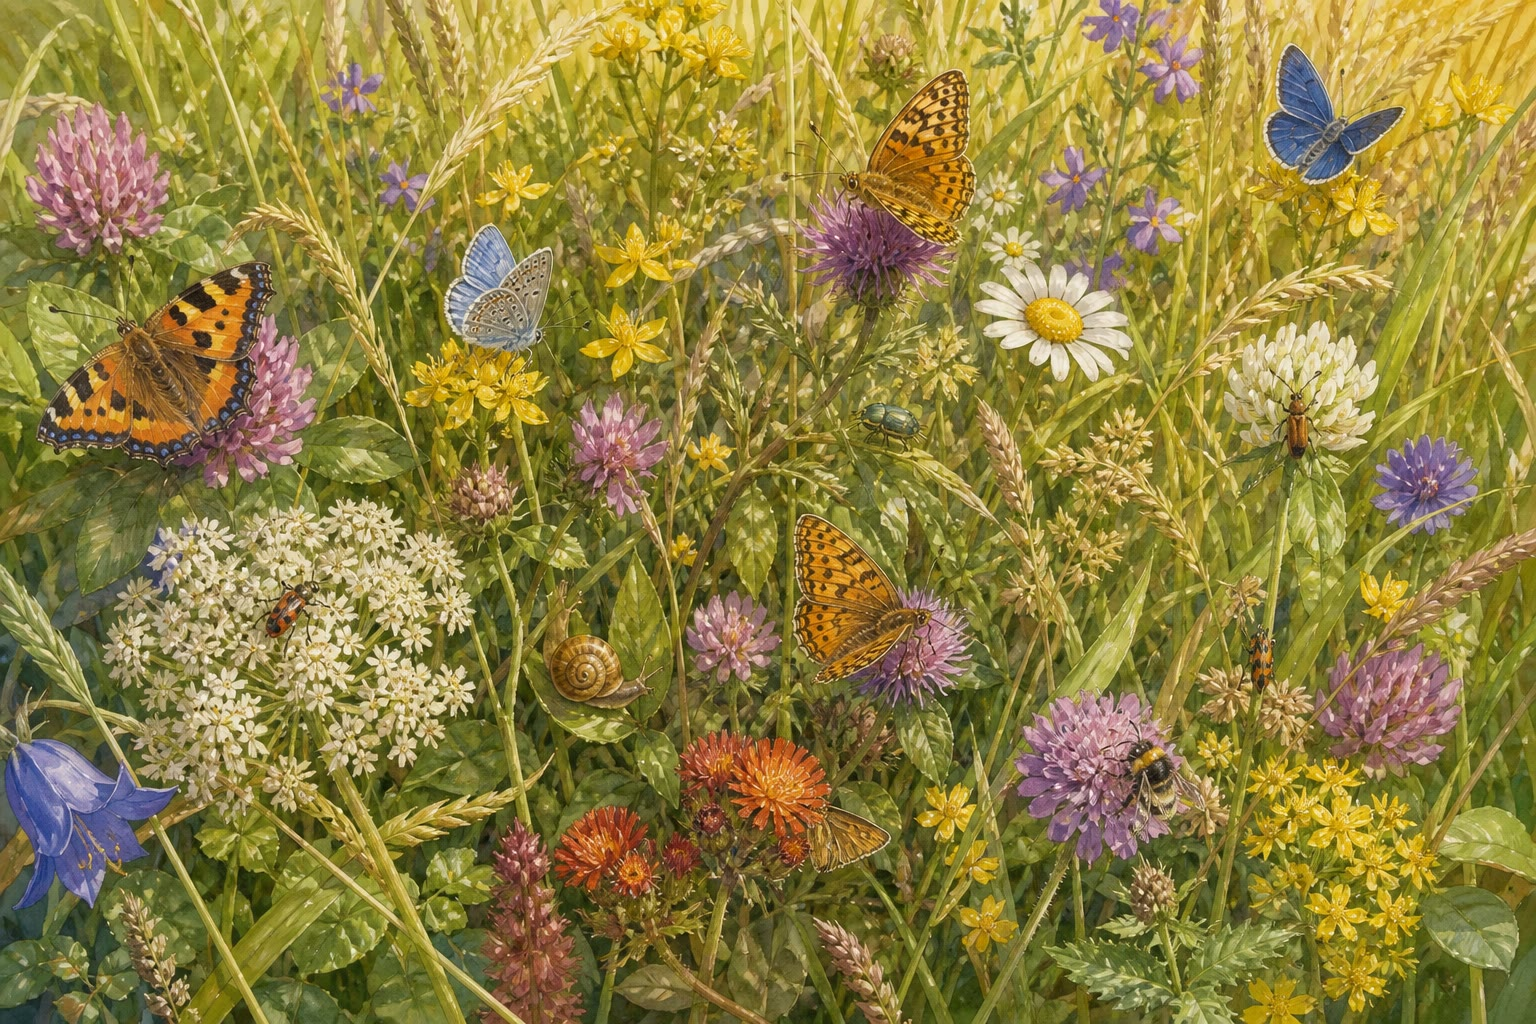
\includegraphics[width=0.62\linewidth]{images/book1/ai/g5-biodiversity-meadow.jpg}

{\small 一平方米草地，正在清点：草、
花、蝴蝶、甲虫、一只蜗牛——而清点
才刚刚开始。}
\end{omfigure}

\begin{example}[清点地球上的物种]\label{ex:g5:biodiversity:planet}
迄今为止，科学家已命名约两百万个\omterm{def:g5:biodiversity:species}{物种}——
并确信这只是总数的一部分，因为每次
认真的考察都会发现新\omterm{def:g5:biodiversity:species}{物种}：甲虫尤其多
（没有哪个类群已命名的\omterm{def:g5:biodiversity:species}{物种}比它更多），还有鱼、青蛙、
\omterm{def:g1:plants-around-us:plant}{植物}，甚至偶尔还有\omterm{prop:g3:sorting-living-things:groups}{哺乳动物}。地球上的\omterm{def:g5:biodiversity:species}{物种}
总数仍不清楚——多数估计认为，比已命名的
\omterm{def:g5:biodiversity:species}{物种}多出数百万个。
\end{example}

\begin{remark}[各尺度上的多样性]\label{rem:g5:biodiversity:scales}
\omterm{def:g5:biodiversity:biodiversity}{生物多样性}同时体现在多个尺度上：一个
\omterm{def:g2:where-animals-live:habitat}{栖息地}中有许多\omterm{def:g5:biodiversity:species}{物种}；许多不同的\omterm{def:g2:where-animals-live:habitat}{栖息地}并列存在（池塘、
树篱、草地——每个都有自己的\omterm{def:g5:biodiversity:species}{物种}，正如
\cref{ex:g2:where-animals-live:four}所示）；在同一\omterm{def:g5:biodiversity:species}{物种}内部，
没有两个个体完全相同——没有两只花园
蜗牛背着完全相同的壳。多样之中有多样，
多样之中又有多样。
\end{remark}

\section{生物多样性为何重要}

\begin{proposition}[网需要它的丝线]\label{prop:g5:biodiversity:web}
同一\omterm{def:g2:where-animals-live:habitat}{栖息地}的\omterm{def:g5:biodiversity:species}{物种}彼此取食、庇护、传粉、
彼此清理——它们是同一张网上的丝线
（见\cref{rem:g3:food-chains:web}）。丝线众多的网能吸收冲击：
若一种猎物\omterm{def:g5:biodiversity:species}{物种}衰减，它的捕食者
就改吃其他\omterm{def:g5:biodiversity:species}{物种}。丝线稀少的网则容易断裂：每失去
一个\omterm{def:g5:biodiversity:species}{物种}，留下的幸存者选择就更少。\omterm{def:g5:biodiversity:biodiversity}{生物多样性}是
网的力量所在。
\end{proposition}
\admitted

\begin{example}[果园的考验]\label{ex:g5:biodiversity:orchard}
一座果园，有树篱、野花带和老树，
栖息着数十种帮手\omterm{def:g5:biodiversity:species}{物种}：蜜蜂和食蚜蝇
为\omterm{def:g1:plants-around-us:parts}{花朵}传粉，
（见\cref{rem:g3:flowers-fruits-seeds:bees}），瓢虫吃掉
蚜虫，\omterm{prop:g3:sorting-living-things:groups}{鸟类}巡逻寻找\omterm{ex:g2:animals-grow-up:butterfly}{毛毛虫}，蚯蚓
使土壤保持疏松。若挖掉树篱、割去花草，
这些帮手就会离开——果农便只能独自
承担它们的工作，而这些工作原本是食物网免费完成的。
\end{example}

\begin{example}[人类依赖食物网生存]\label{ex:g5:biodiversity:people}
人类所吃的一切，都可追溯到\omterm{def:g1:living-or-not:living}{生物}\omterm{def:g5:biodiversity:species}{物种}
（见\cref{rem:g4:what-plants-need:everyone}）；我们的大多数药物
最初都是从\omterm{def:g1:plants-around-us:plant}{植物}、霉菌和其他\omterm{def:g1:living-or-not:living}{生物}中发现的；
棉花、羊毛、木材和皮革，都是\omterm{def:g5:biodiversity:species}{物种}的
产物。食物网的丝线穿过每一个
厨房、药房和衣柜。
\end{example}

\section{生物多样性可能丧失——也可以得到帮助}

\begin{proposition}[多样性如何丧失]\label{prop:g5:biodiversity:loss}
当一个\omterm{def:g5:biodiversity:species}{物种}所依赖的东西被夺走时，它就会减少：
\begin{itemize}
  \item 它的\emph{\omterm{def:g2:where-animals-live:habitat}{栖息地}}被破坏——例如
        \cref{prop:g2:where-animals-live:loss}中被排干的池塘、
        被挖掉的树篱、被硬化的草地；
  \item 它的\omterm{def:g2:caring-for-nature:environment}{环境}遭到污染——垃圾和化学品
        （见\cref{prop:g2:caring-for-nature:harm}）；
  \item 被过度获取——过度捕捞、过度采摘、
        过度猎杀。
\end{itemize}
若某\omterm{def:g5:biodiversity:species}{物种}完全消失——在各处、永远消失——即为
\emph{灭绝}\index{灭绝}。\omterm{prop:g5:biodiversity:loss}{灭绝}不像输掉的
比赛：没有下一局。
\end{proposition}
\admitted

\begin{method}[从小处做起，帮助生物多样性]\label{met:g5:biodiversity:help}
\cref{met:g2:caring-for-nature:rules}中的做法
可以推广到更大范围：
\begin{enumerate}
  \item 保留并种植多样的\omterm{def:g1:plants-around-us:plant}{植物}——五丛灌木
        组成的树篱胜过篱笆，一条花带胜过裸露的碎石地；
  \item 留出野生的角落：枯木、落叶堆、未割的
        草地，都是\omterm{def:g2:where-animals-live:habitat}{栖息地}
        （见\cref{ex:g2:caring-for-nature:home}）；
  \item 帮助这些帮手：巢箱、\omterm{prop:g3:sorting-living-things:groups}{昆虫}庇护所，还有一
        哪怕再小的池塘
        （见\cref{ex:g2:where-animals-live:schoolpond}）；
  \item 年复一年地数一数身边有哪些\omterm{def:g1:living-or-not:living}{生物}——
        被数过的东西才会被注意到，被注意到的东西才会
        得到保护。
\end{enumerate}
\end{method}

\begin{example}[鹳鸟的回归]\label{ex:g5:biodiversity:storks}
湿草甸得到恢复、巢台架起之后，
鹳鸟——曾在整片地区几近绝迹——又飞了回来，
在此繁殖。随之回来的还有青蛙、蜻蜓和草甸上的
花。当那些联系被重新系上时，\omterm{def:g5:biodiversity:species}{物种}便会回归：
保护是有效的，其成果
在村里的广场上便能看到。
\end{example}

\section{练习}

\begin{exercise}[$\star$]\label{exo:g5:biodiversity:1}
什么是\omterm{def:g5:biodiversity:species}{物种}？请从本章中举出三个例子。
\end{exercise}

\begin{exercise}[$\star$]\label{exo:g5:biodiversity:2}
什么是\omterm{def:g5:biodiversity:biodiversity}{生物多样性}？比较草甸与铺装的院子。
\end{exercise}

\begin{exercise}[$\star$]\label{exo:g5:biodiversity:3}
目前已命名的\omterm{def:g5:biodiversity:species}{物种}大约有多少种？为什么真实的
数目一定更多？
\end{exercise}

\begin{exercise}[$\star$]\label{exo:g5:biodiversity:4}
请指出
在\cref{rem:g5:biodiversity:scales}中提到的三种多样性尺度，各举一例。
\end{exercise}

\begin{exercise}[$\star$]\label{exo:g5:biodiversity:5}
为什么\omterm{def:g5:biodiversity:species}{物种}丰富的食物网比
贫乏的食物网更能抵御冲击？请用“猎人改捕其他猎物”这一论证作答。
\end{exercise}

\begin{exercise}[$\star$]\label{exo:g5:biodiversity:6}
列出果园里四种“帮手”\omterm{def:g5:biodiversity:species}{物种}及其各自免费承担的
工作。
\end{exercise}

\begin{exercise}[$\star$]\label{exo:g5:biodiversity:7}
说出\omterm{def:g5:biodiversity:species}{物种}衰退的三种方式，各举一例，
并说明\emph{\omterm{prop:g5:biodiversity:loss}{灭绝}}是什么意思？
\end{exercise}

\begin{exercise}[$\star$]\label{exo:g5:biodiversity:8}
动手试一试：数一数你在户外选定的一小块方形区域中的\omterm{def:g5:biodiversity:species}{物种}，
包括\omterm{def:g1:plants-around-us:plant}{植物}和\omterm{def:g1:animals-around-us:animal}{动物}，已命名的或只被描述过的都算。
再数一数一块铺装的方形区域作为对照。你的两个数字
就是一次\omterm{def:g5:biodiversity:biodiversity}{生物多样性}测量。
\end{exercise}

\begin{exercise}[$\star\star$]\label{exo:g5:biodiversity:9}
“在成千上万个甲虫\omterm{def:g5:biodiversity:species}{物种}中失去一种，
不可能有什么影响。”请用
\cref{prop:g5:biodiversity:web}——并结合
“没有人知道某一\omterm{def:g5:biodiversity:species}{物种}所维系的全部联系”这一事实作答。
\end{exercise}

\begin{exercise}[$\star\star$]\label{exo:g5:biodiversity:10}
鹳鸟的故事被称为\emph{\omterm{def:g2:where-animals-live:habitat}{栖息地}}保护的成功，
而非逐只保护鹳鸟的成功。
请解释二者的区别，并运用
\cref{prop:g2:where-animals-live:loss}，以及与鹳鸟同时回归的
\omterm{def:g1:living-or-not:living}{生物}。
\end{exercise}

\begin{exercise}[$\star\star\star$]\label{exo:g5:biodiversity:11}
一位果园管理者用围栏和碎石取代了树篱和花带，
随后不得不租用蜂箱来传粉，
还得喷药防治蚜虫——为那些原本免费的工作花钱。
请运用\cref{ex:g5:biodiversity:orchard}，
解释实际上被移除的究竟是什么——以及为什么
自然免费工作的“账”通常只有在其停止之后才会显现出来。
\end{exercise}
